\documentclass{beamer}

\usepackage{polyglossia}

\usepackage[orientation = portrait, size = a1, scale = 1.4]{beamerposter}
\usepackage[backend = biber, style = iso-authoryear, sortlocale = en_US, autolang = other, bibencoding = UTF8]{biblatex}
\usepackage{datetime}
\usepackage{adjustbox}
%\usepackage[utf8]{inputenc}
\usepackage{fontspec}
\usepackage{microtype}
\usepackage{listings}
\usepackage{booktabs}

\setdefaultlanguage{english}
\setmainfont{TeX Gyre Termes}
\usetheme{gemini}
\usecolortheme{mit}

\usepackage{tikz}
\usepackage{pgfplots}
\usetikzlibrary{arrows,automata,shapes,calc, patterns, backgrounds}
\input{images/tikzlib}

\definecolor{gray}{rgb}{0.5,0.5,0.5}
\definecolor{mauve}{rgb}{0.58,0,0.82}
\lstset{basicstyle={\small\ttfamily},
	belowskip=3mm,
	breakatwhitespace=true,
	breaklines=true,
	classoffset=0,
	columns=flexible,
	framexleftmargin=0.25em,
	frameshape={}{}{}{}, %To remove to vertical lines on left, set `frameshape={}{}{}{}`
	keywordstyle=\color{blue},
	numbers=none, %If you want line numbers, set `numbers=left`
	numberstyle=\color{gray},
	showstringspaces=false,
	stringstyle=\color{mauve},
	tabsize=3,
	xleftmargin =1em
}


\addbibresource{zotero.bib}
\AtBeginBibliography{\small}

\title{Representation learning for structured data}

\author{%
	Marek Dědič\inst{1 2}
}
\institute{%
	\inst{1} Czech Technical University in Prague \samelineand
	\inst{2} Cisco Systems, Inc.
}

\footercontent{%
	DC @ ECAI 2025, Bologna, Italy \hfill
	\href{mailto:marek@dedic.eu}{marek@dedic.eu}
}

% \logoright{\includegraphics[height=7cm]{logo1.pdf}}
% \logoleft{\includegraphics[height=7cm]{logo2.pdf}}

% If you have N columns, choose \sepwidth and \colwidth such that
% (N+1)*\sepwidth + N*\colwidth = \paperwidth
\newlength{\sepwidth}
\newlength{\colwidth}
\setlength{\sepwidth}{0.033\paperwidth}
\setlength{\colwidth}{0.45\paperwidth}
\newcommand{\separatorcolumn}{\begin{column}{\sepwidth}\end{column}}

\newcommand{\corr}{(\Letter)}
\newcommand{\name}[1]{\textit{#1}}
\newcommand{\mathfield}{\ensuremath{\mathbb}}
\newcommand{\mathmat}{\ensuremath{\mathbf}}
\newcommand{\mathset}{\ensuremath{\mathbb}}
\newcommand{\mathspace}{\ensuremath{\mathcal}}
\newcommand{\mathvec}{\ensuremath{\bm}}

\newcommand{\method}{CSP}
\newcommand{\methodlong}{Convolutional Signal Propagation}
\newcommand{\U}{V} % set of nodes in hypergraph
\newcommand{\uu}{v} % node in hypergraph
\newcommand{\V}{E} % set of hyperedges in hypergraph
\newcommand{\vv}{e} % hyperedge in hypergraph
\newcommand{\HG}{\mathcal{H}} % hypergraph
\newcommand{\HH}{\mathmat{H}} % incidence matrix
\newcommand{\BG}{\mathcal{G}_\mathrm{bip}} % bipartite graph
\newcommand{\E}{E_\mathrm{bip}} % set of edges in bipartite graph
\newcommand{\D}{\mathmat{D}_v} % node degree matrix
\newcommand{\B}{\mathmat{D}_e} % hyperedge degree matrix
\newcommand{\X}{\mathmat{X}} % feature matrix
\newcommand{\Y}{\mathmat{Y}} % label matrix
\newcommand{\y}{y} % label
\newcommand{\x}{\mathvec{x}} % feature vector
\newcommand{\Tr}{V_\mathrm{train}} % Training set
\newcommand{\vdeg}{\mathrm{d}} % degree of node or edge
\newcommand{\edeg}{\delta} % degree of node or edge

\begin{document}
\begin{frame}[fragile,t]

\begin{columns}[t]
	\separatorcolumn

	\begin{column}{\colwidth}
		\begin{block}{The performance-complexity trade-off}
			Graph neural networks (GNNs) suffer from high computational demands, which may be a prohibitive issue in some applications. We investigate the interplay of graph coarsening and the performance of a downstream task. The main aim of this work is to explore the performance-complexity characteristics in the context of graph learning.
			\begin{figure}
				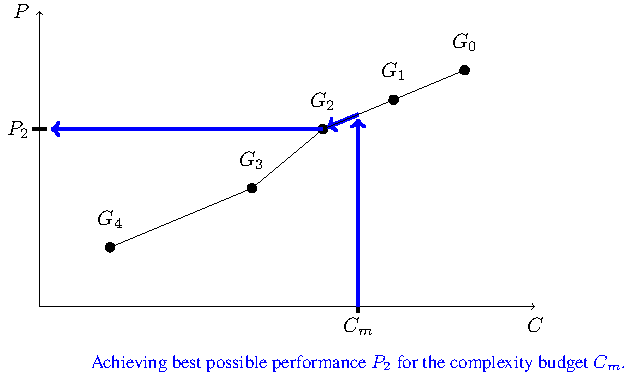
\includegraphics[width=0.8\linewidth]{images/performance-complexity/performance-complexity.pdf}
			\end{figure}
		\end{block}

		\begin{block}{HARP pipeline overview}
			Our work builds on the HARP method for pretraining on coarsened graphs.
			\begin{figure}
				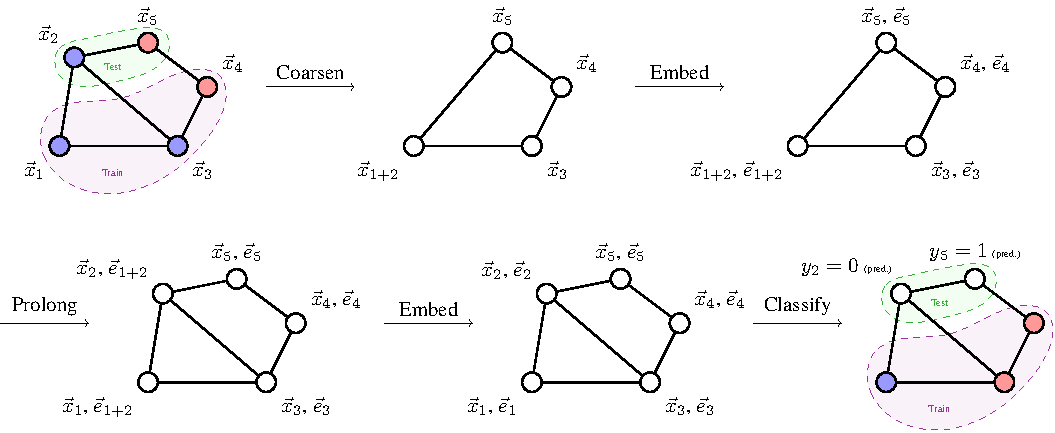
\includegraphics[width=\linewidth]{images/harp-overview/harp-overview.pdf}
			\end{figure}
		\end{block}

		\begin{block}{Adaptive prolongation}
			The main contribution of this work is the adaptive prolongation schema. The algorithm works with the pre-coarsened graphs produced by HARP, however, the prolongation steps are decoupled from the coarsening steps.
			\begin{figure}
				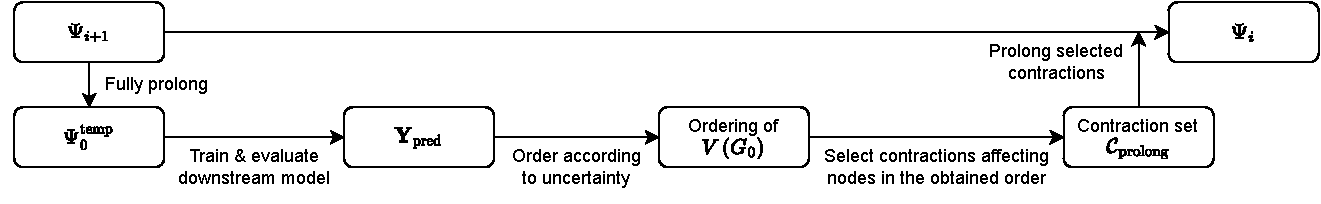
\includegraphics[width=\linewidth]{images/adaptive-prolongation/adaptive-prolongation.pdf}
			\end{figure}
		\end{block}

		\begin{block}{Results}
			\begin{figure}
				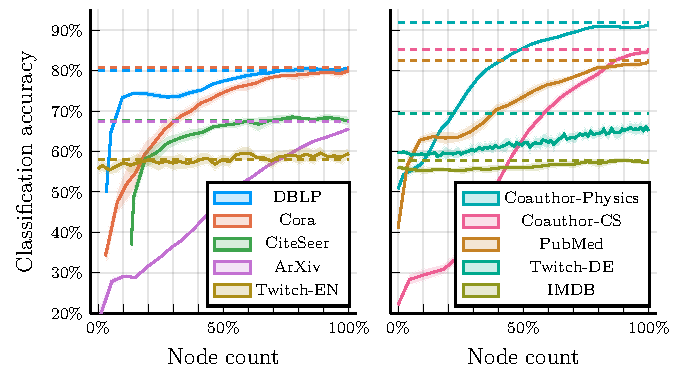
\includegraphics[width = 0.95\linewidth]{images/adaptive-coarsening/adaptive-coarsening.pdf}
			\end{figure}
		\end{block}

		\begin{block}{Motivation -- Hunting for Malicious Entities in Network}
			\input{images/motivation_poster}

			Need for a simple, flexible, well scaling algorithm for efficient entity retrieval.
		\end{block}

		\begin{block}{Intuition}
			\begin{tikzpicture}
\tikzset{node/.style={draw,circle}}
\tikzset{edge/.style={draw,rectangle,inner sep=2pt}}

\tikzset{nodepos/.style={draw,circle, fill=red!20!white}}
\tikzset{nodestress/.style={draw,circle, ultra thick}}




%% Bipartite Graph
\begin{scope}[node distance=2.4cm, circle, draw=black]
    \node[nodepos] at (0, -2) (x1) {$\uu_1$};
    \node[nodepos, below of=x1] (x2) {$\uu_2$};
    \node[nodestress, below of=x2] (x3) {$\uu_3$};
    \node[node, below of=x3] (x4) {$\uu_4$};
    \node[node, below of=x4] (x5) {$\uu_5$};
\end{scope}
    
\begin{scope}[node distance=3.2cm]
    \node[node] at (4, -2) (e1) {$\vv_1$};
    \node[node, below of=e1] (e2) {$\vv_2$};
    \node[node, below of=e2] (e3) {$\vv_3$};
    \node[node, below of=e3] (e4) {$\vv_4$};
\end{scope}

  \draw (e1) -- (x3);
  \draw (e1) -- (x1);
  \draw (e1) -- (x2);
  \draw (e2) -- (x2);
  \draw (e2) -- (x1);
  \draw (e4) -- (x1);
  \draw (e1) -- (x5);
  \draw (e2) -- (x4);
  \draw (e4) -- (x3);
  \draw (e3) -- (x4);
  \draw (e3) -- (x5);


    






%% Hyper-Graph

\begin{scope}[xshift=11cm, yshift=-7cm]
    \node[nodepos] at (0:4) (xx2) {$\uu_2$};
    \node[nodepos] at (72:4)(xx1) {$\uu_1$};
    \node[nodestress] at (144:4)(xx3) {$\uu_3$};
    \node[node] at (216:4)(xx5) {$\uu_5$};
    \node[node] at (288:4)(xx4) {$\uu_4$};

\end{scope}

  %\draw (ee1) -- (xx3);
  %\draw (ee1) -- (xx1);
  %\draw (ee1) -- (xx2);
  %\draw (ee2) -- (xx2);
  %\draw (ee2) -- (xx1);
  %\draw (ee4) -- (xx1);
  %\draw (ee1) -- (xx5);
  %\draw (ee2) -- (xx4);
  %\draw (ee4) -- (xx3);
  %\draw (ee3) -- (xx4);
  %\draw (ee3) -- (xx5);

\begin{scope}[fill opacity=0.2]
    \filldraw[fill=yellow!20] ($(xx1)+(1,0)$) 
        to[out=90,in=0] ($(xx1) + (0,1)$) 
        to[out=180,in=70] ($(xx3) + (-1,0)$) 
        to[out=250,in=210] ($(xx3) + (0,-1)$)
        to[out=30,in=270] ($(xx1) + (1,0)$);
    \filldraw[fill=green!20] ($(xx5)+(-1,0)$) 
        to[out=250,in=180] ($(xx5) + (0,-1)$) 
        to[out=0,in=210] ($(xx4) + (0,-1)$) 
        to[out=30,in=290] ($(xx4) + (1, 0)$)
        to[out=110,in=70] ($(xx5) + (-1,0)$);
    \filldraw[fill=cyan!20] ($(xx1)+(-1,0)$) 
        to[out=270,in=90] ($(xx4) + (-1,0)$) 
        to[out=270,in=180] ($(xx4) + (0,-1)$) 
        to[out=0,in=270] ($(xx2) + (1,0)$) 
        to[out=90,in=0] ($(xx1) + (0, 1)$)
        to[out=180,in=90] ($(xx1) + (-1, 0)$);
    \filldraw[fill=gray!20] ($(xx1)+(0,1)$) 
        to[out=180,in=90] ($(xx3) + (-1,0)$) 
        to[out=270,in=210] ($(xx5) + (0,-1)$) 
        to[out=30,in=270] ($(xx2) + (1,0)$) 
        to[out=90,in=0] ($(xx1) + (0, 1)$);
\end{scope}


\begin{scope}[xshift=20cm, yshift=-3cm]
\node at (0,0) {%
    $\mathmat{H}=\left[\begin{array}{cccc}
 1 & 1 & 0 & 1 \\
 1 & 1 & 0 & 0 \\
 1 & 0 & 0 & 1 \\
 0 & 1 & 1 & 0 \\
 1 & 0 & 1 & 0 
     \end{array}
     \right]$
};

\end{scope}

\begin{scope}[xshift=20cm, yshift=-9cm]
\node at (0,0) {%
     $\mathmat{Y}=\left[\begin{array}{c}
 1 \\
 1 \\
 0 \\
 0 \\
 0 
     \end{array}
     \right]$
};

\end{scope}

\end{tikzpicture}

		\end{block}

		\begin{block}{Basic Definition of CSP}
			\begin{equation*}
				\hspace*{-1.5cm}
				x_k^{(l+1)} = \underbrace{\frac{1}{deg\left( \uu_k \right)}\sum_{\substack{j \\ \uu_k \in \vv_j}}}_{\mathrm{2nd~step}} \ \underbrace{\frac{1}{deg \left( \vv_j \right)}\sum_{\substack{i \\ \uu_i \in \vv_j}} x_i^{(l)}}_{\mathrm{1st~step}}
				,\quad \mathmat{X}^{(l+1)} = \underbrace{\D^{-1} \HH}_{\mathrm{2nd~step}} \ \underbrace{\B^{-1} \HH^T \mathmat{X}^{(l)}}_{\mathrm{1st~step}}
			\end{equation*}

			SQL implementation (1 layer):
			\begin{lstlisting}[language=SQL,numbers=left,basicstyle=\small]
SELECT nodeId, AVG(y) AS updatedX FROM (
	SELECT nodeId, AVG(X) OVER (PARTITION BY edgeId) AS y
	FROM graph)
GROUP BY nodeId;
			\end{lstlisting}
		\end{block}

		\begin{block}{Comparison with Other Methods}
			\begin{itemize}
				\item Naive Bayes
					\begin{itemize}
						\item Fitting binomial Naive Bayes in the 1st step ($\B^{-1} \HH^T \mathmat{X}^{(l)}$)
						\item Simple mean instead of Bayes rule in the 2nd step
					\end{itemize}
				\item Hyper-Graph Convolutional Network (HGCN)
					\begin{equation*}
						\mathmat{X}^{(l+1)} = \sigma(\D^{−1} \HH \mathmat{W} \B^{−1} \HH^T \mathmat{X}^{(l)} \boldsymbol{\Theta}),
					\end{equation*}
					where \( \mathmat{W} \) and \( \boldsymbol{\Theta} \) are realized as non-learnable identity matrices.
				\item Label Propagation
					\begin{equation*}
						\mathmat{Y}^{(l+1)} = \alpha \D^{−1} \mathmat{A} \mathmat{Y}^{(l)} + \left( 1 - \alpha \right) \mathmat{Y}^{(l)}
					\end{equation*}
					with $\HH \B^{-1} \HH^T = \frac{1}{2}( \mathmat{A} + \D)$,
					\begin{equation*}
						\mathmat{X}^{(l+1)} = \frac{1}{2} \D^{-1} \mathmat{A} \mathmat{X}^{(l)} + \frac{1}{2} \mathmat{X}^{(l)}.
					\end{equation*}
			\end{itemize}
		\end{block}
\end{column}

\separatorcolumn

\begin{column}{\colwidth}
	\begin{alertblock}{Key takeaways}
		\begin{itemize}
			\item CSP is a very simple learning method for classification and retrieval on graphs, hyper-graphs or problems described by one-hot features.
			\item CSP can be written in just few lines of SQL code.
			\item CSP shown as: 1) a natural extension of label propagation algorithm to hyper-graphs, 2) a special case of forward pass of Hyper-GCN, 3) an alternative way of binomial Naive Bayes inference.
			\item CSP achieves comparable performance to reference methods in multiple problems, while being significantly cheaper to compute.
		\end{itemize}
	\end{alertblock}

	\begin{block}{Evaluated Applications}
		\adjustbox{width=\columnwidth}{%
			\begin{tabular}{llllllll}
				\textbf{Dataset} & \textbf{Node} & \textbf{Node label} & \textbf{Hyper-edge} & \textbf{\#nodes} & \textbf{\#hyper-edges} & \textbf{\#bip.\ edges} & \textbf{\#classes}\\
				\midrule
				Cora-CA & paper & topic & author & 2708 & 1072	& 4585 & 7\\
				Cora-CC & paper & topic & co-cited papers & 2708 & 1579  & 4786 &7\\
				CiteSeer & paper & topic & co-cited papers& 3312 & 1079  & 3453 &6\\
				DBLP & paper & topic & author& 41302 & 22363 & 99561 & 6\\
				PubMed & paper & topic & co-cited papers& 19717 & 7963	& 34629 &3\\
				Corona & text & sentiment & token& 44955 & 998	& 3455918 &5\\
				movie-RA & movie & category & user& 62423 & 162541 & 25000095 &20\\
				movie-TA & movie & category & tag& 62423 & 14592  & 1093360 &20\\
				\bottomrule
			\end{tabular}
		}
	\end{block}

	\begin{block}{Experiment Setup}
		\begin{itemize}
			\item Tasks related to each class:
				\begin{itemize}
					\item Binary classification (90\% train, 10\% test)
					\item Retrieval (10\% train, 90\% test)
				\end{itemize}
			\item Considered methods:
				\begin{itemize}
					\item Convolutional Signal Propagation (1,2 and 3 layers)
					\item Naive Bayes operating with one-hot features
					\item Random forest, logistic regression, HGCN with NMF
				\end{itemize}
		\end{itemize}
	\end{block}

	\begin{block}{Binary Classification Results -- Average ROC-AUC}
		\adjustbox{width=\columnwidth}{%
			\begin{tabular}{lrrrrrrrr}
				\textbf{Method} & \textbf{CiteSeer} & \textbf{Cora-CA} & \textbf{Cora-CC} & \textbf{DBLP} & \textbf{PubMed} & \textbf{Corona} & \textbf{movie-RA} & \textbf{movie-TA} \\
				\midrule
				\textbf{\method{} 1-layer} & \underline{0.646} & \underline{0.882} & 0.716 & \underline{0.968} & 0.537 & \textbf{0.704} & \underline{0.789} & \underline{0.717} \\
				\textbf{\method{} 2-layer} & 0.630 & \underline{0.872} & 0.686 & \underline{0.972} & 0.518 & 0.618 & 0.700 & \underline{0.697} \\
				\textbf{\method{} 3-layer} & 0.613 & 0.862 & 0.655 & \underline{0.972} & 0.516 & 0.580 & 0.640 & 0.673 \\
				\textbf{Naive Bayes} & \textbf{0.686} & \textbf{0.913} & \underline{0.775} & \textbf{0.974} & \textbf{0.633} & \textbf{0.704} & \underline{0.753} & 0.557 \\
				\textbf{HGCN-NMF} & \underline{0.659} & 0.832 & \textbf{0.786} & 0.775 & \underline{0.624} & 0.622 & \underline{0.794} & \textbf{0.724} \\
				\textbf{LR-NMF} & 0.604 & 0.794 & 0.703 & 0.705 & 0.556 & 0.647 & \underline{0.754} & \underline{0.675} \\
				\textbf{RF-NMF} & \underline{0.667} & \underline{0.897} & \underline{0.772} & 0.905 & \underline{0.623} & 0.617 & \textbf{0.797} & \underline{0.691} \\
				\textbf{Random} & 0.499 & 0.505 & 0.489 & 0.501 & 0.502 & 0.503 & 0.499 & 0.487 \\
				\bottomrule
			\end{tabular}
		}
	\end{block}

	\begin{block}{Retrieval Results -- P@{}100}
		\adjustbox{width=\columnwidth}{%
			\begin{tabular}{lrrrrrrrr}
				\textbf{Method} & \textbf{CiteSeer} & \textbf{Cora-CA} & \textbf{Cora-CC} & \textbf{DBLP} & \textbf{PubMed} & \textbf{Corona} &\textbf{movie-RA} & \textbf{movie-TA} \\
				\midrule
				\textbf{\method{} 1-layer} & 0.494 & \underline{0.703} & 0.530 & 0.869 & 0.798 & \textbf{0.530} & 0.334 & 0.156 \\
				\textbf{\method{} 2-layer} & \underline{0.558} & \underline{0.718} & \underline{0.681} & 0.865 & \underline{0.826} & 0.440 & 0.336 & 0.186 \\
				\textbf{\method{} 3-layer} & \textbf{0.568} & \textbf{0.721} & \textbf{0.707} & 0.869 & \underline{0.850} & 0.332 & 0.238 & 0.186 \\
				\textbf{Naive Bayes} & 0.471 & \underline{0.686} & 0.491 & \textbf{0.951} & \underline{0.860} & 0.446 & 0.216 & 0.153 \\
				\textbf{HGCN-NMF} & 0.482 & \underline{0.671} & 0.607 & 0.794 & \textbf{0.871} & 0.392 & 0.257 & 0.148 \\
				\textbf{LR-NMF} & 0.329 & 0.603 & 0.372 & 0.602 & 0.735 & 0.397 & \textbf{0.580} & \textbf{0.356} \\
				\textbf{RF-NMF} & 0.303 & 0.474 & 0.482 & 0.843 & 0.794 & 0.381 & 0.470 & 0.131 \\
				\textbf{Random} & 0.153 & 0.132 & 0.129 & 0.155 & 0.308 & 0.180 & 0.040 & 0.055 \\
				\bottomrule
			\end{tabular}
		}
	\end{block}

	\begin{block}{Execution Time in Microseconds}
		\adjustbox{width=\columnwidth}{%
			\begin{tabular}{lrrrrrrrr}
				\textbf{Method} & \textbf{CiteSeer} & \textbf{Cora-CA} & \textbf{Cora-CC} & \textbf{DBLP} & \textbf{PubMed} & \textbf{Corona} & \textbf{movie-RA} & \textbf{movie-TA} \\
				\midrule
				\textbf{\method{} 1-layer} & \textbf{1.35} & \textbf{1.23} & \textbf{1.24} & \textbf{3.51} & \textbf{4.01} & \textbf{22.83} & 170.63 & \textbf{12.07} \\
				\textbf{\method{} 2-layer} & 2.41 & 2.25 & 2.24 & 7.46 & 7.35 & 47.39 & 349.67 & 25.88 \\
				\textbf{\method{} 3-layer} & 3.31 & 3.09 & 3.08 & 9.65 & 9.1 & 70.98 & 506.1 & 35.75 \\
				\textbf{Naive Bayes} & 2.59 & 2.73 & 2.54 & 11.16 & 5.35 & 89.3 & 1 051.53 & 35.61 \\
				\textbf{*HGCN-NMF} & 23 714 & 23 690 & 23 709 & 29 123 & 23 879 & 112 314 & 620 717 & 70 778 \\
				\textbf{*LR-NMF} & 44.45 & 51.59 & 49.54 & 64.96 & 44.69 & 56 & \textbf{61.82} & 74.07 \\
				\textbf{*RF-NMF} & 140.76 & 143.85 & 134.52 & 1 148.83 & 323.6 & 1 608.58 & 697.85 & 716.68 \\
				\bottomrule
			\end{tabular}
		}
		\footnotesize{*NMF processing is not included in evaluation of the time duration.}
	\end{block}

	\begin{block}{Asymptotic Complexity}
		\adjustbox{width=\columnwidth}{%
			\begin{tabular}{lccccc}
				\textbf{\method{}} & \textbf{Naive Bayes} & \textbf{HGCN} & \textbf{LR} & \textbf{RF} \\
				\midrule
				\( \mathcal{O} \left( d \left( \Sigma_\U + \Sigma_\V \right) \right) \) & \( \mathcal{O} \left( n m \left\lvert \Tr \right\rvert \right) \)  & \( \mathcal{O} \left( T \Sigma_\V h d \right) \)  & \( \mathcal{O} \left( d \left\lvert \Tr \right\rvert \right) \)	& \( \mathcal{O} \left( d \log{d} \left\lvert \Tr \right\rvert \right) \) \\
				\bottomrule
			\end{tabular}
		}
	\end{block}

	%\begin{block}{Convolutional Signal Propagation Variants}
	%\begin{itemize}
	%	 \item normalization
	%	 \begin{itemize}
	%		 \item column-wise $\X^{(l+1)} = \HH \B^{-1} \HH^T \D^{-1} \X^{(l)}$
	%		 \item symmetric $\X^{(l+1)} = \D^{-1/2} \HH \B^{-1} \HH^T \D^{-1/2} \X^{(l)}.$
	%	 \end{itemize}
	%	 \item general $\alpha \in (0,1)$: $\X^{(l+1)} = 2 \alpha \D^{-1} \HH \B^{-1} %\HH^T \X^{(l)} + \left( 1 - 2 \alpha \right) \X^{(l)}$
	%\end{itemize}
	%\end{block}
\end{column}

\separatorcolumn
\end{columns}

\end{frame}
\end{document}
